\documentclass[10pt,border=4pt]{standalone}
\usepackage{mathptmx}
\usepackage{amsmath,amssymb,bm}
\usepackage{tikz}
\usetikzlibrary{patterns,decorations.pathmorphing,decorations.pathreplacing,arrows.meta,fit,backgrounds,calc,positioning,shapes.geometric}
\definecolor{acc}{HTML}{0B5394}
\definecolor{accl}{HTML}{EAF0F7}
\definecolor{grp}{HTML}{F5F5F5}
\definecolor{org}{HTML}{C55A11}
\definecolor{orgl}{HTML}{FBEFE6}
\tikzset{
 dat/.style={draw=black,line width=0.6pt,fill=white,align=center,font=\small,inner sep=3pt,minimum height=0.85cm},
 lay/.style={draw=acc,line width=0.8pt,fill=accl,rounded corners=2pt,align=center,font=\small,inner sep=3pt,minimum height=0.85cm},
 cnd/.style={draw=org,line width=0.8pt,fill=orgl,rounded corners=2pt,align=center,font=\small,inner sep=3pt,minimum height=0.75cm},
 op/.style={circle,draw=black,line width=0.6pt,fill=white,inner sep=0.5pt,font=\small,minimum size=5mm},
 grpb/.style={draw=black!45,dashed,line width=0.6pt,rounded corners=3pt,inner sep=6pt},
 arr/.style={-{Latex[length=2.2mm,width=1.7mm]},line width=0.7pt},
 carr/.style={-{Latex[length=2.2mm,width=1.7mm]},line width=0.7pt,draw=org},
 shp/.style={font=\scriptsize,text=black!70,inner sep=1pt},
 lab/.style={font=\footnotesize,inner sep=1pt},
 ttl/.style={font=\small\bfseries,inner sep=0pt,anchor=west}
}
\newcommand{\xh}{\mathbf{x}_h}\newcommand{\xf}{\mathbf{x}_f}

\begin{document}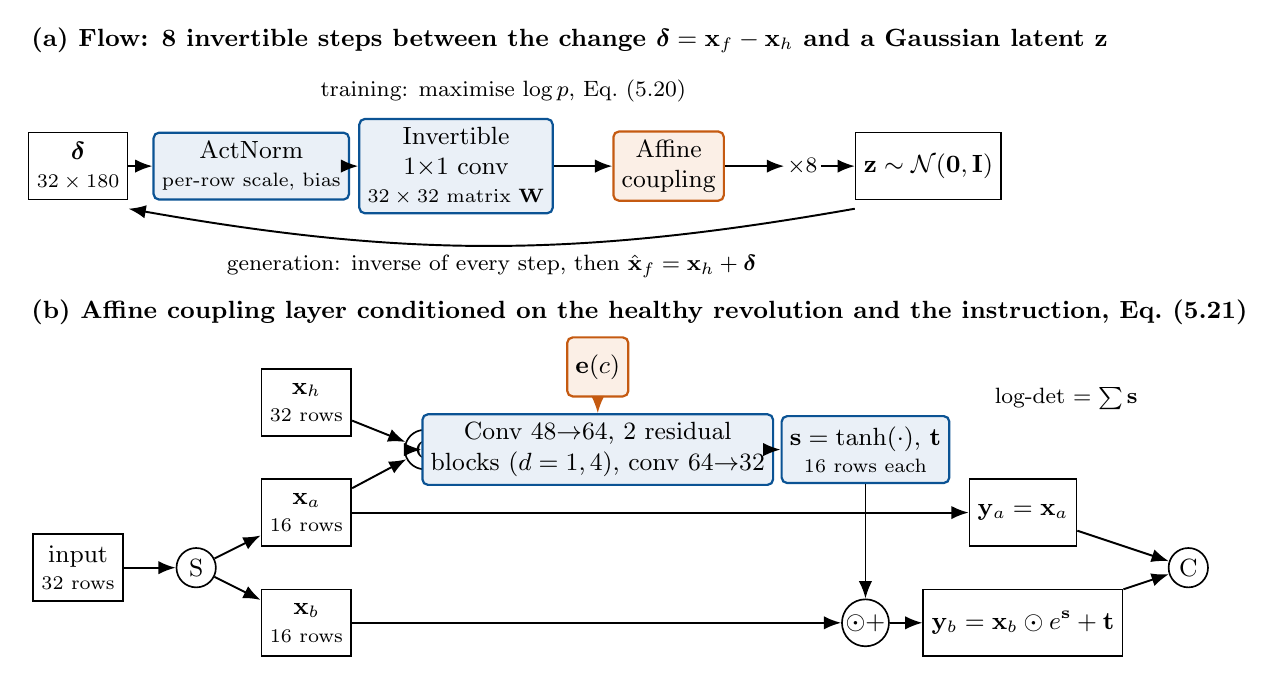
\begin{tikzpicture}[x=1cm,y=1cm]
\node[ttl] at (-0.6,1.6) {(a) Flow: 8 invertible steps between the change $\boldsymbol\delta=\xf-\xh$ and a Gaussian latent $\mathbf{z}$};
\node[dat] (d) at (0,0) {$\boldsymbol\delta$\\[-1pt]\scriptsize $32\times180$};
\node[lay] (an) at (2.2,0) {ActNorm\\[-1pt]\scriptsize per-row scale, bias};
\node[lay] (iv) at (4.8,0) {Invertible\\$1{\times}1$ conv\\[-1pt]\scriptsize $32\times32$ matrix $\mathbf{W}$};
\node[lay,draw=org,fill=orgl] (cp) at (7.5,0) {Affine\\coupling};
\node[lab] (rep) at (9.2,0) {$\times 8$};
\node[dat] (z) at (10.8,0) {$\mathbf{z}\sim\mathcal{N}(\mathbf{0},\mathbf{I})$};
\draw[arr] (d)--(an); \draw[arr] (an)--(iv); \draw[arr] (iv)--(cp); \draw[arr] (cp)--(rep); \draw[arr] (rep)--(z);
\draw[arr] ([yshift=-3pt]z.south west) to[bend left=10] node[lab,below=2pt]{generation: inverse of every step, then $\hat{\mathbf{x}}_f=\xh+\boldsymbol\delta$} ([yshift=-3pt]d.south east);
\node[lab] at (5.4,0.95) {training: maximise $\log p$, Eq.~(5.20)};
% (b) coupling layer
\node[ttl] at (-0.6,-1.85) {(b) Affine coupling layer conditioned on the healthy revolution and the instruction, Eq.~(5.21)};
\node[dat] (in) at (0,-5.10) {input\\[-1pt]\scriptsize 32 rows};
\node[op] (sp) at (1.5,-5.10) {S};
\node[dat] (xa) at (2.9,-4.40) {$\mathbf{x}_a$\\[-1pt]\scriptsize 16 rows};
\node[dat] (xb) at (2.9,-5.80) {$\mathbf{x}_b$\\[-1pt]\scriptsize 16 rows};
\node[op] (cat) at (4.4,-3.60) {C};
\node[dat] (xh) at (2.9,-3.00) {$\xh$\\[-1pt]\scriptsize 32 rows};
\node[lay] (net) at (6.6,-3.60) {Conv $48{\to}64$, 2 residual\\blocks ($d=1,4$), conv $64{\to}32$};
\node[cnd] (e) at (6.6,-2.55) {$\mathbf{e}(c)$};
\node[lay] (st) at (10.0,-3.60) {$\mathbf{s}=\tanh(\cdot)$, $\mathbf{t}$\\[-1pt]\scriptsize 16 rows each};
\node[op] (aff) at (10.0,-5.80) {$\odot{+}$};
\node[dat] (yb) at (12.0,-5.80) {$\mathbf{y}_b=\mathbf{x}_b\odot e^{\mathbf{s}}+\mathbf{t}$};
\node[dat] (ya) at (12.0,-4.40) {$\mathbf{y}_a=\mathbf{x}_a$};
\node[op] (cc) at (14.1,-5.10) {C};
\draw[arr] (in)--(sp); \draw[arr] (sp)--(xa); \draw[arr] (sp)--(xb); \draw[arr] (xa)--(cat); \draw[arr] (xh)--(cat); \draw[arr] (cat)--(net); \draw[carr] (e)--(net); \draw[arr] (net)--(st); \draw[arr] (st)--(aff);
\draw[arr] (xb)--(aff); \draw[arr] (aff)--(yb); \draw[arr] (xa)--(ya); \draw[arr] (ya)--(cc); \draw[arr] (yb)--(cc);
\node[lab,align=left,anchor=west] at (11.6,-2.95) {log-det $=\sum\mathbf{s}$};
\end{tikzpicture}\end{document}
